% Networks graphs
\subsection{Networks/Graphs} \label{s:lit:graph_overview}

Genes impact each other, and there is a relationship between different subsets that give rise to pathways necessary for various functions in the tissue. The key aspect in genetics is the interdependence between elements. Traditional clustering analysis such as hierarchical clustering does not take these relationships into account, partly due to the fact that they are unknown, and that the computational models do not have that layer of information built-in. Co-expressed networks are one way to model such connections by computing the pairwise correlation of gene expression to determine the strength of connections; the research done in this area is presented in \cref{s:lit:co_net}. The gene relationships can be represented in a graph or network, where a node (or vertex) represents a gene and an edge represents the connection between them (see \cref{fig:graphs_basic}).

\begin{figure}[!htb]
  \centering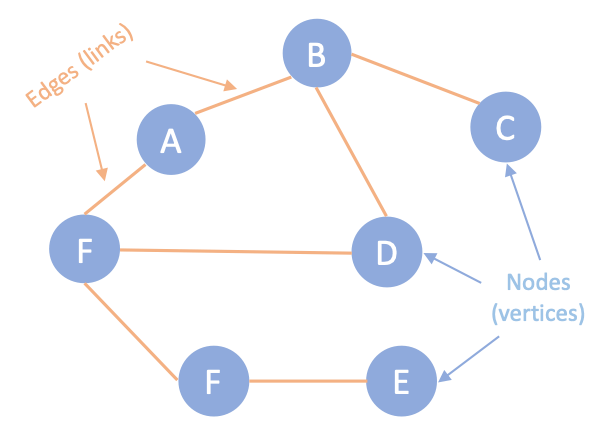
\includegraphics[width=0.5\textwidth,height=0.5\textheight,keepaspectratio]{Sections/Lit_review/Resources/basic_graphs.png}
    \caption{Basic graphs illustrating gene interactions.}
    \label{fig:graphs_basic}
\end{figure}

To establish how genes are linked and interact in a network, the edges are assigned values that reinforce the links between nodes (genes). Data that can be tabulated and processed by various graph algorithms while the edges weights represent an opportunity to model the different data types available in the omics. The work on integrating multiple data type in networks/graphs is covered in \cref{s:lit:net_data_int}.

One aspect of graph analysis is to identify influential nodes, which in biology could involve finding genes that have a significant impact on the network, such as Transcription Factors (TFs). Another aspect of network theory, extensively explored in \cref{s:lit:comm_detect}, involves examining nodes (i.e., genes) that can be grouped together. Graphs are an effective and intuitive tool for visualising and navigating high-dimensional data.

The challenge with graphs is that they are less developed and can be computationally taxing. For example, community detection is a hot topic because there is no established method for identifying groups of nodes, and some popular methods can find patterns in noise. These issues are discussed at length in \cref{s:lit:comm_detect}.

\subsection{Networks - metrics} \label{s:lit:networks_metrics}
